% ============================================================
%  Guia de Usuario -- Sistema de Biblioteca UCR Recinto Grecia
%  Autores: Marcos Ferreto Estrada, Paulo Anchia Correas
%  Compilar: pdflatex guia_usuario.tex  (ejecutar 2 veces)
% ============================================================
\documentclass[12pt, a4paper]{article}

% --- Codificacion y fuente ----------------------------------
\usepackage[utf8]{inputenc}
\usepackage[T1]{fontenc}
\usepackage{lmodern}

% --- Idioma (nueva API de babel, compatible con TeX Live 2023+) -
\usepackage{babel}
\babelprovide[import, main]{spanish}

% --- Paquetes esteticos y utiles ----------------------------
\usepackage{geometry}
\usepackage{graphicx}
\usepackage{xcolor}
\usepackage{titlesec}
\usepackage{fancyhdr}
\usepackage{enumitem}
\usepackage{booktabs}
\usepackage{array}
\usepackage{tabularx}
\usepackage{float}
\usepackage{microtype}
\usepackage{hyperref}

% --- Geometria de pagina ------------------------------------
\geometry{
  top    = 2.5cm,
  bottom = 2.5cm,
  left   = 2.8cm,
  right  = 2.8cm,
  headheight = 15pt
}

% --- Paleta de colores UCR ----------------------------------
\definecolor{UCRBlue}  {HTML}{2471A3}
\definecolor{UCRDark}  {HTML}{1B2631}
\definecolor{UCRPanel} {HTML}{3D5166}
\definecolor{UCRGreen} {HTML}{1E8449}
\definecolor{UCRRed}   {HTML}{922B21}
\definecolor{NoteBlue} {HTML}{D6EAF8}
\definecolor{TipGreen} {HTML}{D5F5E3}
\definecolor{WarnYell} {HTML}{FDEBD0}

% --- Hipervinculos ------------------------------------------
\hypersetup{
  colorlinks = true,
  linkcolor  = UCRBlue,
  urlcolor   = UCRBlue,
  pdftitle   = {Guia de Usuario - Sistema de Biblioteca UCR},
  pdfauthor  = {Marcos Ferreto Estrada, Paulo Anchias Correas},
}

% --- Encabezado y pie de pagina ----------------------------
\pagestyle{fancy}
\fancyhf{}
\fancyhead[L]{\small\color{UCRBlue}\textbf{Biblioteca UCR -- Recinto de Grecia}}
\fancyhead[R]{\small\color{gray}Guía de Usuario}
\fancyfoot[C]{\small\color{gray}\thepage}
\renewcommand{\headrulewidth}{0.4pt}

% --- Estilos de secciones ----------------------------------
\titleformat{\section}
  {\Large\bfseries\color{UCRBlue}}
  {\thesection.}{0.5em}{}
  [\vspace{-4pt}\rule{\linewidth}{1.2pt}]

\titleformat{\subsection}
  {\large\bfseries\color{UCRDark}}
  {\thesubsection.}{0.5em}{}

\titleformat{\subsubsection}
  {\normalsize\bfseries\color{UCRPanel}}
  {\thesubsubsection.}{0.5em}{}

% --- Cajas informativas (lrbox + minipage) ---------------
\newsavebox{\mybox}

\newenvironment{notebox}{%
  \vspace{6pt}\par\noindent
  \begin{lrbox}{\mybox}%
    \begin{minipage}{\dimexpr\linewidth-16pt\relax}%
      \noindent\textcolor{UCRBlue}{\textbf{Nota:}}\ %
}{%
    \end{minipage}%
  \end{lrbox}%
  \setlength{\fboxsep}{8pt}%
  \colorbox{NoteBlue}{\usebox{\mybox}}%
  \vspace{6pt}\par%
}

\newenvironment{tipbox}{%
  \vspace{6pt}\par\noindent
  \begin{lrbox}{\mybox}%
    \begin{minipage}{\dimexpr\linewidth-16pt\relax}%
      \noindent\textcolor{UCRGreen}{\textbf{Consejo:}}\ %
}{%
    \end{minipage}%
  \end{lrbox}%
  \setlength{\fboxsep}{8pt}%
  \colorbox{TipGreen}{\usebox{\mybox}}%
  \vspace{6pt}\par%
}

\newenvironment{warnbox}{%
  \vspace{6pt}\par\noindent
  \begin{lrbox}{\mybox}%
    \begin{minipage}{\dimexpr\linewidth-16pt\relax}%
      \noindent\textcolor{UCRRed}{\textbf{Advertencia:}}\ %
}{%
    \end{minipage}%
  \end{lrbox}%
  \setlength{\fboxsep}{8pt}%
  \colorbox{WarnYell}{\usebox{\mybox}}%
  \vspace{6pt}\par%
}

% --- Estilos de tabla ---------------------------------------
\renewcommand{\arraystretch}{1.35}

% --- Comandos de botones y campos ---------------------------
\newcommand{\boton}[1]{%
  \fcolorbox{UCRBlue}{UCRBlue}{\color{white}\small\textbf{\ #1\ }}%
}
\newcommand{\botonrojo}[1]{%
  \fcolorbox{UCRRed}{UCRRed}{\color{white}\small\textbf{\ #1\ }}%
}
\newcommand{\botonverde}[1]{%
  \fcolorbox{UCRGreen}{UCRGreen}{\color{white}\small\textbf{\ #1\ }}%
}
\newcommand{\campo}[1]{\texttt{\textbf{#1}}}

% ============================================================
\begin{document}
% ============================================================

% ============================================================
%  PORTADA
% ============================================================
\begin{titlepage}
  \centering
  \vspace*{1.2cm}

  % Logo institucional
  
\includegraphics[width=6cm]{../gui/iconos/firma-promocional-con-texto-negro.png}

  \vspace{1.4cm}
  \rule{\linewidth}{2pt}\\[0.5em]
  {\Huge\bfseries\color{UCRBlue} Sistema de Biblioteca}\\[0.3em]
  {\LARGE\bfseries\color{UCRDark} Recinto de Grecia}\\[0.4em]
  \rule{\linewidth}{2pt}

  \vspace{1cm}
  {\Large\bfseries Guía de Usuario}

  \vspace{2cm}
  \begin{tabular}{@{}ll@{}}
    \toprule
    \textbf{Proyecto}    & Biblioteca UCR --- Recinto de Grecia \\
    \textbf{Curso}       & Estructuras de Datos \\
    \midrule
    \textbf{Integrantes} & Marcos Ferreto Estrada \\
                         & Paulo Anchía Correás   \\
    \midrule
    \textbf{Versión}     & 1.0 \\
    \textbf{Fecha}       & Junio 2026 \\
    \bottomrule
  \end{tabular}

  \vfill
  {\small\color{gray}%
    Universidad de Costa Rica \textbullet{} Sede de Occidente \textbullet{} Recinto de Grecia}
\end{titlepage}

% --- Indice de contenidos ----------------------------------
\tableofcontents
\newpage

% ============================================================
%  1. INTRODUCCION
% ============================================================
\section{Introducción}

El \textbf{Sistema de Biblioteca UCR -- Recinto de Grecia} es una aplicación de escritorio
desarrollada en Python con la biblioteca gráfica \textit{Tkinter}.
Su objetivo es facilitar la gestión integral de libros, estudiantes y préstamos del recinto.

La aplicación emplea tres estructuras de datos avanzadas para garantizar eficiencia:

\begin{itemize}[leftmargin=1.8cm]
  \item \textbf{Árbol AVL} --- gestión y búsqueda de libros, ordenados por código.
        Complejidad de búsqueda: \textit{O(log n)}.
  \item \textbf{Tabla Hash} --- acceso rápido a estudiantes mediante su número de carnet.
        Tiempo promedio: \textit{O(1)}.
  \item \textbf{Árbol Rojo-Negro} --- registro y listado de préstamos activos,
        ordenados por código de préstamo.
\end{itemize}

Los datos se persisten automáticamente en archivos \textbf{XML}, conservando
la información entre sesiones.

\begin{notebox}
Esta guía está orientada al personal de biblioteca.
No se requiere conocimiento técnico previo para operar el sistema.
\end{notebox}

% ============================================================
%  2. REQUISITOS Y ARRANQUE
% ============================================================
\section{Requisitos del Sistema y Arranque}

\subsection{Requisitos mínimos}
\begin{itemize}
  \item Sistema operativo: Linux, Windows o macOS.
  \item Python 3.10 o superior.
  \item Dependencias del archivo \texttt{pyproject.toml} instaladas.
\end{itemize}

\subsection{Cómo iniciar la aplicación}

Desde una terminal, situado en la carpeta raíz del proyecto, ejecute:

\begin{center}
  \ttfamily python main.py
\end{center}

Al iniciar, el sistema carga los datos desde los archivos XML.
La barra de estado inferior mostrará el número de libros cargados en el sistema.

\begin{tipbox}
Si usa el entorno virtual del proyecto, actívelo primero:\\[4pt]
Linux/macOS: \texttt{source .venv/bin/activate}\\
Windows: \texttt{.venv\textbackslash Scripts\textbackslash activate}
\end{tipbox}

% ============================================================
%  3. DESCRIPCION GENERAL DE LA INTERFAZ
% ============================================================
\section{Descripción General de la Interfaz}

\begin{figure}[H]
  \centering
  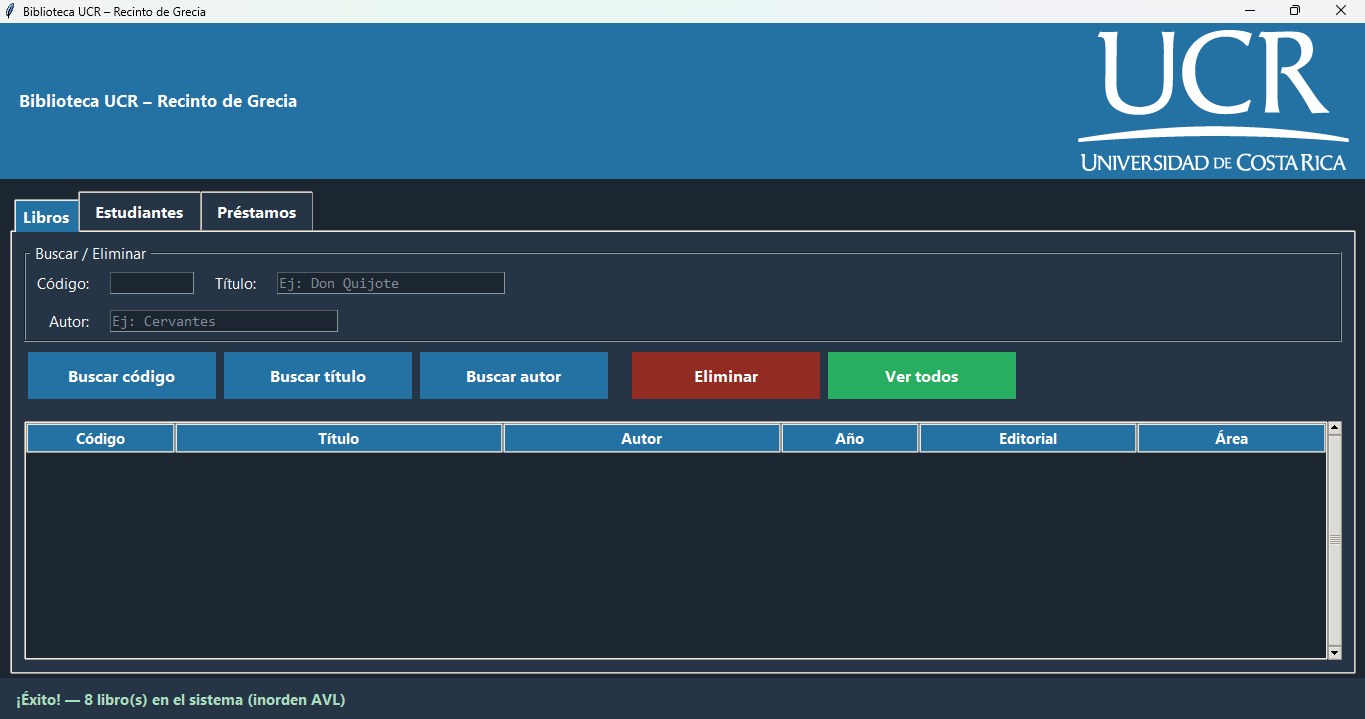
\includegraphics[width=0.92\textwidth]{img/tab_libros.png}
  \caption{Ventana principal del sistema --- pestaña \textit{Libros}.}
  \label{fig:vista-general}
\end{figure}

La ventana principal (1160 $\times$ 660 px) se divide en tres zonas:

\begin{enumerate}
  \item \textbf{Encabezado} --- banda azul superior con el título del sistema
        y el logo institucional de la UCR.
  \item \textbf{Área de pestañas} --- contiene las funcionalidades de
        \textit{Libros}, \textit{Estudiantes} y \textit{Préstamos}.
  \item \textbf{Barra de estado} --- franja inferior que informa en tiempo real
        el resultado de cada operación.
\end{enumerate}

\subsection{Convención de colores de los botones}

\begin{center}
  \begin{tabular}{>{\centering\arraybackslash}m{3.5cm} m{9.5cm}}
    \toprule
    \textbf{Color}       & \textbf{Significado} \\
    \midrule
    \boton{Azul}         & Operaciones de búsqueda (solo consulta, sin modificar datos). \\[6pt]
    \botonrojo{Rojo}     & Eliminar registros (acción destructiva, requiere confirmación). \\[6pt]
    \botonverde{Verde}   & Confirmar un préstamo o listar todos los registros. \\
    \bottomrule
  \end{tabular}
\end{center}

\subsection{Barra de estado}

La barra inferior cambia de color según el resultado de la última acción:

\begin{itemize}
  \item \textcolor{UCRGreen}{\textbf{Verde}} (\textit{¡Éxito! ---}) operación completada correctamente.
  \item \textcolor{UCRRed}{\textbf{Rojo}} (\textit{¡Error! ---}) se detectó un problema.
\end{itemize}

La barra también indica la estructura de datos utilizada:
\texttt{(AVL)}, \texttt{(Hash)} o \texttt{(Rojinegro)}.

% ============================================================
%  4. PESTANA LIBROS
% ============================================================
\section{Pestaña: Libros}

\begin{figure}[H]
  \centering
  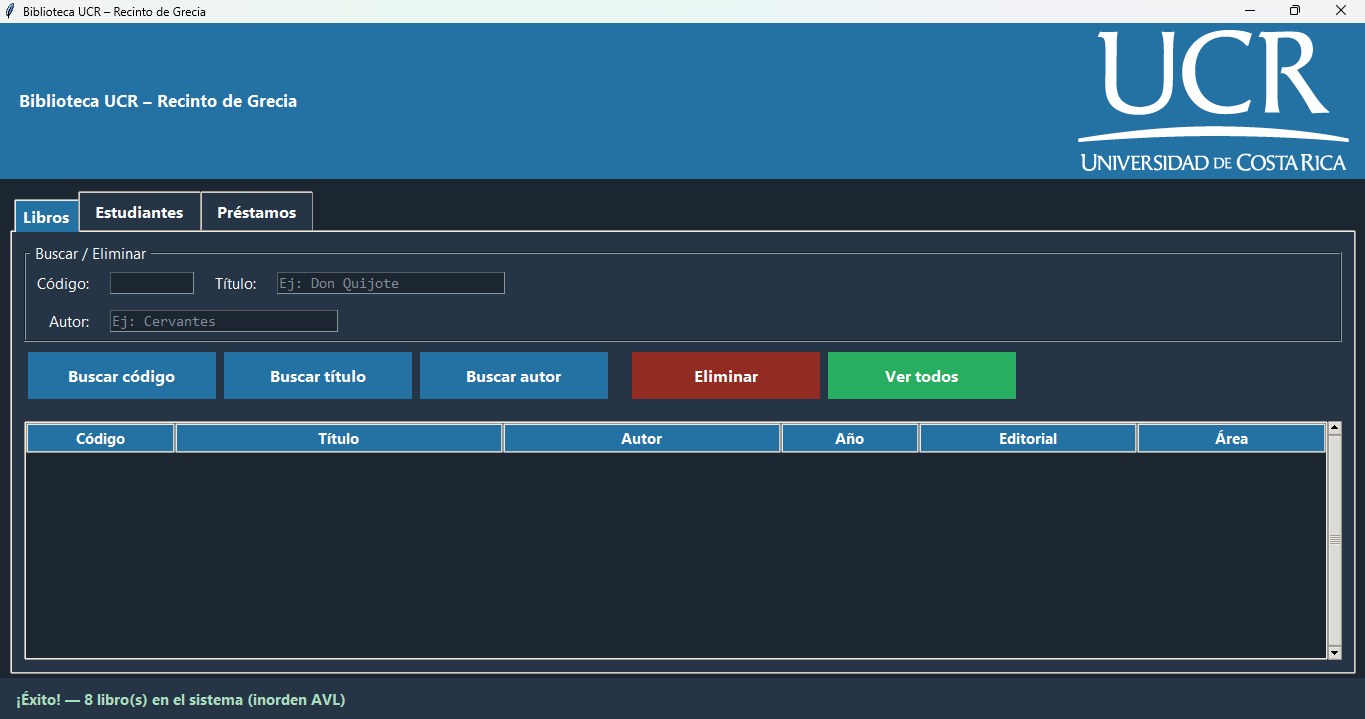
\includegraphics[width=0.92\textwidth]{img/tab_libros.png}
  \caption{Pestaña \textit{Libros}: formulario de búsqueda y tabla de resultados.}
  \label{fig:tab-libros}
\end{figure}

Esta pestaña permite \textbf{buscar} y \textbf{eliminar} libros del catálogo.
Los resultados aparecen en una tabla con las siguientes columnas:

\begin{center}
  \begin{tabular}{ll}
    \toprule
    \textbf{Columna} & \textbf{Descripción} \\
    \midrule
    Código    & Identificador numérico único del libro. \\
    Título    & Nombre completo del libro. \\
    Autor     & Nombre del autor o autores. \\
    Año       & Año de publicación. \\
    Editorial & Casa editorial. \\
    Área      & Categoría temática (ej.\ Ciencias, Literatura). \\
    \bottomrule
  \end{tabular}
\end{center}

\subsection{Campos de búsqueda}

\begin{itemize}
  \item \campo{Código} --- Número entero del libro (Ej: \texttt{101}).
  \item \campo{Título} --- Nombre del libro (Ej: \texttt{Don Quijote}).
  \item \campo{Autor} --- Apellido o nombre del autor (Ej: \texttt{Cervantes}).
\end{itemize}

\begin{notebox}
Los campos muestran texto guía en gris (placeholder) que desaparece al hacer clic.
No es necesario rellenar todos los campos; solo el que corresponda a la búsqueda.
\end{notebox}

\subsection{Botones disponibles}

\begin{center}
  \begin{tabularx}{\textwidth}{>{\centering\arraybackslash}m{4cm} X}
    \toprule
    \textbf{Botón} & \textbf{Función} \\
    \midrule
    \boton{Buscar código} &
      Busca en el Árbol AVL el libro cuyo código coincida exactamente
      con el valor del campo \campo{Código}. \\[4pt]
    \boton{Buscar título} &
      Busca en el Árbol AVL el libro con el título indicado. \\[4pt]
    \boton{Buscar autor} &
      Lista todos los libros del autor especificado. \\[4pt]
    \botonrojo{Eliminar} &
      Elimina el libro con el código ingresado.
      Solicita confirmación antes de proceder. \\[4pt]
    \botonverde{Ver todos} &
      Muestra todos los libros ordenados de forma ascendente
      por código (recorrido \textit{in-orden} del AVL). \\
    \bottomrule
  \end{tabularx}
\end{center}

\subsection{Procedimiento: Buscar un libro por código}

\begin{enumerate}
  \item Haga clic en el campo \campo{Código} y escriba el número (ej.\ \texttt{101}).
  \item Presione \textbf{Enter} o haga clic en \boton{Buscar código}.
  \item El resultado aparece en la tabla inferior.
  \item La barra de estado confirma si el libro fue encontrado.
\end{enumerate}

\subsection{Procedimiento: Eliminar un libro}

\begin{enumerate}
  \item Ingrese el código del libro en \campo{Código}.
  \item Haga clic en \botonrojo{Eliminar}.
  \item En el cuadro de confirmación, haga clic en \textbf{Sí} para confirmar
        o \textbf{No} para cancelar.
  \item Si la eliminación es exitosa, la tabla se actualiza automáticamente.
\end{enumerate}

\begin{warnbox}
Un libro no puede eliminarse si tiene préstamos activos.
El sistema mostrará un error indicando que primero debe registrarse la devolución.
\end{warnbox}

% ============================================================
%  5. PESTANA ESTUDIANTES
% ============================================================
\section{Pestaña: Estudiantes}

\begin{figure}[H]
  \centering
  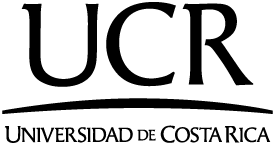
\includegraphics[width=0.92\textwidth]{img/tab_estudiantes.png}
  \caption{Pestaña \textit{Estudiantes}: formulario de búsqueda y tabla de resultados.}
  \label{fig:tab-estudiantes}
\end{figure}

Permite \textbf{buscar} y \textbf{eliminar} registros de estudiantes.
La tabla muestra los siguientes datos:

\begin{center}
  \begin{tabular}{ll}
    \toprule
    \textbf{Columna} & \textbf{Descripción} \\
    \midrule
    Carnet    & Número de identificación único del estudiante. \\
    Nombre    & Nombre completo. \\
    Carrera   & Carrera universitaria que cursa. \\
    Teléfono  & Número de contacto. \\
    Correo    & Dirección de correo electrónico. \\
    Dirección & Lugar de residencia. \\
    \bottomrule
  \end{tabular}
\end{center}

\subsection{Campos de búsqueda}

\begin{itemize}
  \item \campo{Carnet} --- Número entero de identificación (Ej: \texttt{2023001}).
  \item \campo{Nombre} --- Nombre completo del estudiante (Ej: \texttt{Juan Pérez}).
  \item \campo{Carrera} --- Nombre de la carrera (Ej: \texttt{Informática}).
\end{itemize}

\subsection{Botones disponibles}

\begin{center}
  \begin{tabularx}{\textwidth}{>{\centering\arraybackslash}m{4cm} X}
    \toprule
    \textbf{Botón} & \textbf{Función} \\
    \midrule
    \boton{Buscar carnet} &
      Localiza al estudiante con el carnet exacto ingresado.
      Usa la Tabla Hash (\textit{O(1)} promedio). \\[4pt]
    \boton{Buscar nombre} &
      Busca al estudiante por nombre completo en la Tabla Hash. \\[4pt]
    \boton{Buscar carrera} &
      Lista todos los estudiantes matriculados en la carrera indicada. \\[4pt]
    \botonrojo{Eliminar} &
      Elimina el estudiante cuyo carnet está en \campo{Carnet}.
      Solicita confirmación. \\[4pt]
    \botonverde{Ver todos} &
      Muestra todos los estudiantes registrados en el sistema. \\
    \bottomrule
  \end{tabularx}
\end{center}

\subsection{Procedimiento: Buscar un estudiante por carnet}

\begin{enumerate}
  \item Haga clic en el campo \campo{Carnet} e ingrese el número
        (ej.\ \texttt{2023001}).
  \item Presione \textbf{Enter} o haga clic en \boton{Buscar carnet}.
  \item La información completa del estudiante aparece en la tabla.
\end{enumerate}

\subsection{Procedimiento: Eliminar un estudiante}

\begin{enumerate}
  \item Ingrese el carnet en \campo{Carnet}.
  \item Haga clic en \botonrojo{Eliminar}.
  \item Confirme la acción en el cuadro de diálogo.
\end{enumerate}

\begin{warnbox}
Un estudiante no puede eliminarse si tiene préstamos activos.
Primero registre la devolución de todos sus libros prestados.
\end{warnbox}

% ============================================================
%  6. PESTANA PRESTAMOS
% ============================================================
\section{Pestaña: Préstamos}

\begin{figure}[H]
  \centering
  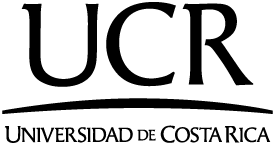
\includegraphics[width=0.92\textwidth]{img/tab_prestamos.png}
  \caption{Pestaña \textit{Préstamos}: formularios para dar y devolver libros.}
  \label{fig:tab-prestamos}
\end{figure}

Esta pestaña centraliza la gestión de préstamos.
Se divide en dos secciones:

\begin{itemize}
  \item \textbf{Dar Préstamo} --- registra la salida de un libro hacia un estudiante.
  \item \textbf{Devolver Libro} --- registra el regreso de un libro prestado.
\end{itemize}

La tabla de préstamos activos muestra:

\begin{center}
  \begin{tabular}{ll}
    \toprule
    \textbf{Columna}  & \textbf{Descripción} \\
    \midrule
    Cod. Préstamo & Identificador único del préstamo. \\
    Cod. Libro    & Código del libro prestado. \\
    Carnet        & Carnet del estudiante que lo tiene. \\
    Fecha         & Fecha en que se realizó el préstamo (AAAA-MM-DD). \\
    Vence         & Fecha límite para la devolución (15 días después). \\
    \bottomrule
  \end{tabular}
\end{center}

\subsection{Dar un préstamo}

\subsubsection{Campos requeridos}

\begin{itemize}
  \item \campo{Cod. libro} --- Código numérico del libro a prestar (Ej: \texttt{101}).
  \item \campo{Carnet} --- Número de carnet del estudiante (Ej: \texttt{2023001}).
\end{itemize}

\subsubsection{Procedimiento}

\begin{enumerate}
  \item Ingrese el código del libro en \campo{Cod. libro}.
        Puede presionar \textbf{Tab} para moverse al siguiente campo.
  \item Ingrese el carnet del estudiante en \campo{Carnet}.
  \item Haga clic en \botonverde{Dar Préstamo} o presione \textbf{Enter}.
  \item El sistema valida que el libro y el estudiante existan,
        registra el préstamo con la fecha actual y actualiza la tabla.
\end{enumerate}

\begin{tipbox}
La fecha de vencimiento se calcula automáticamente sumando \textbf{15 días calendario}
a la fecha del préstamo. Recuerde informar al estudiante la fecha límite.
\end{tipbox}

\subsection{Devolver un libro}

\subsubsection{Campos requeridos}

\begin{itemize}
  \item \campo{Cod. préstamo} --- Código del préstamo, visible en la columna
        \textit{Cod. Préstamo} de la tabla (Ej: \texttt{5}).
\end{itemize}

\subsubsection{Procedimiento}

\begin{enumerate}
  \item Consulte la tabla de préstamos activos con \botonverde{Ver todos}
        para identificar el código del préstamo a devolver.
  \item Ingrese ese código en \campo{Cod. préstamo}.
  \item Haga clic en \boton{Devolver} o presione \textbf{Enter}.
  \item Confirme la acción en el cuadro de diálogo.
  \item El préstamo se elimina y la tabla se actualiza.
\end{enumerate}

\subsection{Ver todos los préstamos}

Haga clic en \botonverde{Ver todos} para listar todos los préstamos activos
ordenados por código (recorrido \textit{in-orden} del Árbol Rojo-Negro).

% ============================================================
%  7. ATAJOS DE TECLADO
% ============================================================
\section{Atajos de Teclado}

\begin{center}
  \begin{tabular}{ll}
    \toprule
    \textbf{Tecla / Acción}    & \textbf{Efecto} \\
    \midrule
    \texttt{Enter}             & Ejecuta la búsqueda o acción del campo activo. \\
    \texttt{Tab}               & Mueve el foco al siguiente campo de entrada. \\
    Clic en pestaña            & Cambia entre \textit{Libros}, \textit{Estudiantes} y \textit{Préstamos}. \\
    \bottomrule
  \end{tabular}
\end{center}

% ============================================================
%  8. MENSAJES DE ERROR COMUNES
% ============================================================
\section{Mensajes de Error Comunes}

\begin{center}
  \begin{tabularx}{\textwidth}{>{\ttfamily\small}p{5.6cm} X}
    \toprule
    \textbf{Mensaje en barra de estado} & \textbf{Causa y solución} \\
    \midrule
    Ingrese un código. &
      El campo \campo{Código} está vacío. Ingresar el número antes de buscar. \\[4pt]
    El código debe ser un número entero. &
      Se escribieron letras o símbolos en un campo numérico. Usar solo dígitos. \\[4pt]
    Libro X no encontrado. &
      El código no corresponde a ningún libro registrado. Verificar el número. \\[4pt]
    No se encontró 'Título'. &
      El título no existe en el catálogo. Revisar la ortografía. \\[4pt]
    No hay libros de 'Autor'. &
      No hay libros de ese autor en el sistema. \\[4pt]
    Ingrese un carnet. &
      El campo \campo{Carnet} está vacío. \\[4pt]
    Estudiante X no encontrado. &
      El carnet no existe. Verificar el número. \\[4pt]
    Ingrese el código del préstamo. &
      El campo \campo{Cod. préstamo} está vacío. \\[4pt]
    Código y carnet deben ser enteros. &
      Se ingresó texto en lugar de números en el formulario de préstamos. \\
    \bottomrule
  \end{tabularx}
\end{center}

% ============================================================
%  9. PERSISTENCIA DE DATOS
% ============================================================
\section{Persistencia de Datos}

El sistema guarda toda la información en archivos XML
dentro de la carpeta \texttt{datos/} del proyecto:

\begin{center}
  \begin{tabular}{ll}
    \toprule
    \textbf{Archivo}         & \textbf{Contenido} \\
    \midrule
    \texttt{libros.xml}      & Catálogo completo de libros. \\
    \texttt{estudiantes.xml} & Registro de todos los estudiantes. \\
    \texttt{prestamos.xml}   & Historial de préstamos activos. \\
    \bottomrule
  \end{tabular}
\end{center}

Cada vez que se registra un préstamo, una devolución o una eliminación,
el archivo XML correspondiente se actualiza de forma automática.

\begin{warnbox}
No elimine ni modifique manualmente los archivos XML.
Hacerlo podría causar errores al iniciar la aplicación.
\end{warnbox}

% ============================================================
%  10. GLOSARIO
% ============================================================
\section{Glosario}

\begin{description}[leftmargin=3.2cm, labelwidth=3cm, style=nextline]
  \item[AVL]
    Árbol binario de búsqueda autobalanceado.
    Garantiza búsquedas, inserciones y eliminaciones en \textit{O(log n)}.
  \item[Árbol Rojo-Negro]
    Árbol binario autobalanceado que gestiona los préstamos,
    ordenados por código de préstamo.
  \item[Tabla Hash]
    Estructura que permite búsquedas de estudiantes en tiempo promedio \textit{O(1)}.
  \item[In-orden]
    Recorrido de un árbol de menor a mayor; produce una lista ordenada.
  \item[Carnet]
    Número de identificación único del estudiante en la UCR.
  \item[Préstamo activo]
    Préstamo registrado que aún no ha sido devuelto.
  \item[XML]
    Formato de archivo de texto estructurado para almacenar los datos.
  \item[Placeholder]
    Texto de ayuda en gris que aparece en un campo vacío.
    Desaparece al hacer clic.
\end{description}

% ============================================================
%  11. INFORMACION DEL PROYECTO
% ============================================================
\section{Información del Proyecto}

\begin{center}
  \begin{tabular}{@{}ll@{}}
    \toprule
    \textbf{Dato}          & \textbf{Detalle} \\
    \midrule
    Nombre del proyecto    & Biblioteca UCR --- Recinto de Grecia \\
    Curso                  & Estructuras de Datos \\
    Desarrolladores        & Marcos Ferreto Estrada \\
                           & Paulo Anchía Correás \\
    Lenguaje               & Python 3 \\
    Biblioteca gráfica     & Tkinter (ttk) \\
    Persistencia           & Archivos XML \\
    Estructuras de datos   & Árbol AVL, Tabla Hash, Árbol Rojo-Negro \\
    Duración del préstamo  & 15 días calendario \\
    \bottomrule
  \end{tabular}
\end{center}

\vfill
\begin{center}
  \small\color{gray}
  Universidad de Costa Rica \textbullet{} Sede de Occidente \textbullet{}
  Recinto de Grecia\\
  \textit{Todos los derechos reservados \textbullet{} 2026}
\end{center}

\end{document}
